\section{Internationale Arbeitsteilung}
\subsection{Komparativer Kostenvorteil}
\begin{multicols}{2}
	Vorgehen:
	\begin{itemize}
		\item Opportunitätskosten berechnen für alle Artikel.
		\item Opportunitätskosten vergleichen.
		\item Der Ort mit den tiefsten Opportunitätskosten produziert und
		exportiert zu einem Preis zwischen Opportunitätskosten im
		Exportort und den Opportunitätskosten im Importort (natürlich nur ohne
		Zölle, Transportkosten etc.).
	\end{itemize}
	Falls Gleichstand ist findet kein Handel statt.
	\includegraphics[width=9cm]{images/h03f07.png}
\end{multicols}

\subsection{Weltmarktpreis}
\begin{description}
	\item[Hoher Weltmarktpreis] inländische Produktion übersteigt den Konsum, dieser Überschuss wird exportiert
	\begin{itemize}
		\item Konsumentenrente $\downarrow$
		\item Produzentenrente $\uparrow$
		\item Gesamtrente $\uparrow$
	\end{itemize}
	\item[Tiefer Weltmarktpreis] inländischer Konsum übersteigt Produktion
	\begin{itemize}
		\item Konsumentenrente $\uparrow$
		\item Produzentenrente $\downarrow$
		\item Gesamtrente $\uparrow$
	\end{itemize}
	\item Internationale Arbeitsteilung bringt positive Wohlfahrtseffekte, unabhängig davon, ob der Weltmarktpreis höher oder tiefer als der Heimmarktpreis ist.
\end{description}
\begin{multicols}{3}
	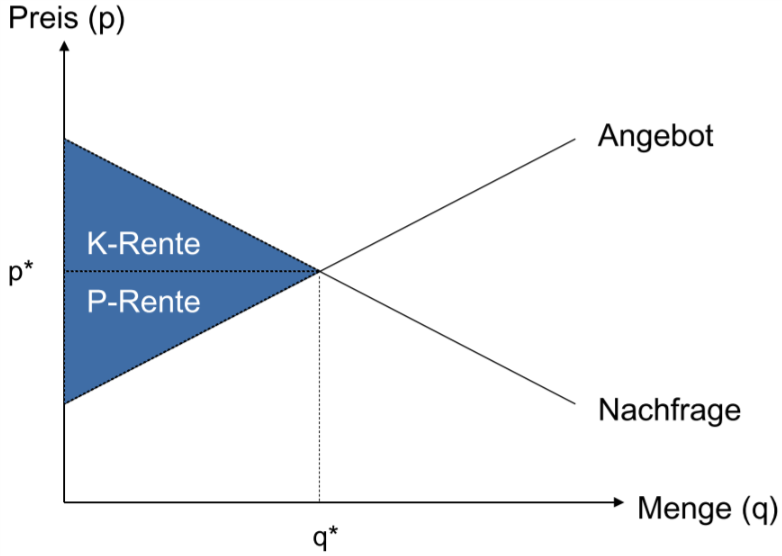
\includegraphics[width=\linewidth]{images/rente.png}
	\columnbreak
	\includegraphics[width=\linewidth]{images/h03f11.png}
	\columnbreak
	\includegraphics[width=\linewidth]{images/h03f13.png}
\end{multicols}

\subsection{Protektionismus (Zölle)}
\begin{minipage}{0.35\linewidth}
	\begin{itemize}
		\item Freihandel bringt eine relativ starke Umverteilung der Wohlfahrt zugunsten des Konsumenten mit sich; dies zu Lasten der Produzenten und des Staates
		\item Der Produzent hat hohes Eigeninteresse, der Konsument nur kleines, daher kann sich oftmals Produzent (Verbände) eher durchsetzen in der Politik
		\item Produzenten sichern sich durch diese Staatseingriffe eine künstliche Rente. Der notwendige Strukturwandel der Wirtschaft wird dadurch verzögert.
	\end{itemize}
\end{minipage}
\begin{minipage}{0.6\linewidth}
		\includegraphics[width=12cm]{images/zolle.png}
\end{minipage}

\subsubsection{Moderne Formen des Protektionismus}
\begin{minipage}{0.35\linewidth}
	Durch Abschaffung von Zöllen durch Organisationen wie WTO weichen Länder immer mehr auf sogenannte $"$nichttarifäre$"$ Handelshemmnisse aus:
\begin{itemize}
	\item Quoten
	\item Technische Handelshemmnisse (Vorschriften die nur in einem Land gelten; inländische Produzenten besser gestellt als ausländische)
	\item Subventionen
	\item Öffentliche Aufträge (Bevorzugung von Inländern)
\end{itemize}
\end{minipage}
\begin{minipage}{0.6\linewidth}
	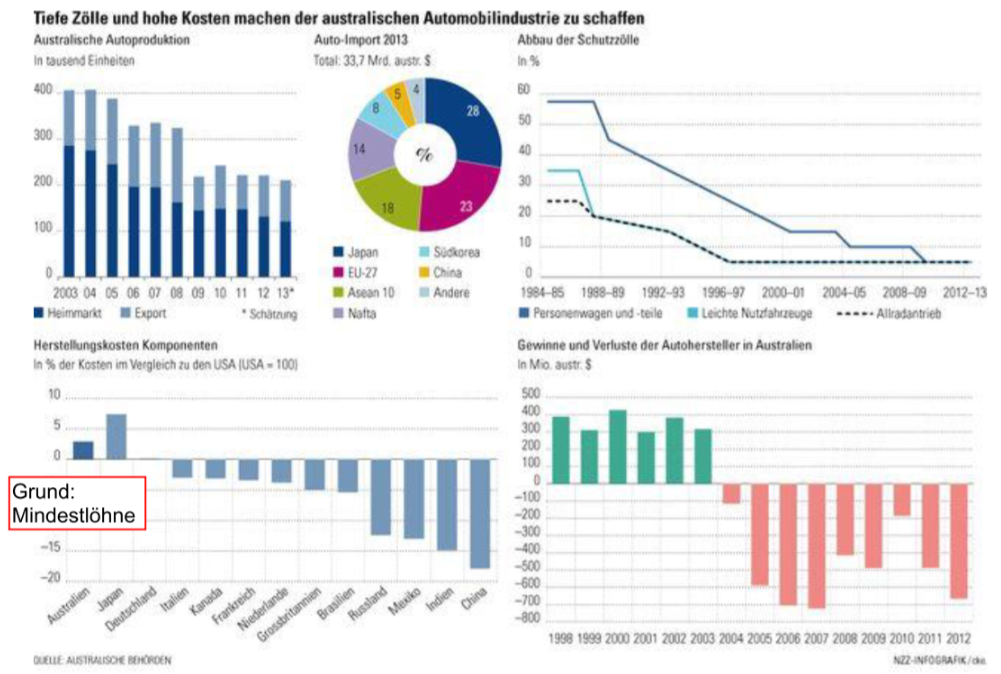
\includegraphics[width=\linewidth]{images/australien.png}
\end{minipage}

\subsection{Handelsliberalisierung}
\begin{minipage}{0.35\linewidth}
	Es gibt drei Formen der internationalen Arbeitsteilung:
	\begin{itemize}
		\item Multilaterale Handelsliberalisierung (z.B. WTO)
		\item Regionale Handelsliberalisierung (z.B. EU)
		\item Bilaterale Handelsliberalisierung (Der "Schweizer"-Weg)
	\end{itemize}
	\vspace{\baselineskip}
	\textbf{Regionale Handelsliberalisierung}\\
	Durch regionale Integration entsteht eine Diskriminierung der Länder, welche nicht Mitglieder des Integrationsraumes sind. Die regionale Integration generiert zusätzlichen Handel, verzerrt diesen aber gleichzeitig. Dadurch entstehen: 
	\begin{itemize}
		\item Handelsschaffung
		\item Handelsumlenkung
	\end{itemize}
\end{minipage}
\begin{minipage}{0.6\linewidth}
	\includegraphics[width=12cm]{images/integrationsraume.png}
\end{minipage}

\begin{minipage}{0.6\linewidth}
	\subsubsection{Formen von Integrationsräumen}
	\includegraphics[width=\linewidth]{images/integrationsformen.png}
\end{minipage}
\begin{minipage}{0.3\linewidth}
	\subsubsection{Übersicht internationale Wirtschaftsorganisationen}
	\textbf{Bretton-Woods-Institutionen}
	\begin{itemize}
		\item IWF (IMF)
		\item Weltbank (World Bank)
	\end{itemize}
	\textbf{Weitere Institutionen}
	\begin{itemize}
		\item WTO
		\item OECD
		\item UNCTAD
		\item G7
		\item G20
	\end{itemize}
\end{minipage}

\subsubsection{Internationale Wirtschaftsorganisationen}
\textbf{IWF/IMF: Internationaler Währungsfond}\\
\begin{itemize}
	\item Sonderorganisation der UNO
	\item Vergabe von Krediten an Länder ohne ausreichende Währungsreserven, die in Zahlungsschwierigkeiten sind
	\begin{itemize}
		\item an wirtschaftspolitische Auflagen geknüpft, um Rückzahlung zu sichern
	\end{itemize}
	\item Förderung der Zusammenarbeit in Währungspolitik
	\item Ausweitung des Welthandels
	\item Stabilisierung von Wechselkursen
	\item Überwachung der Geldpolitik
	\item 189 Mitgliedsstaaten
	\begin{itemize}
		\item Stimmrecht orientiert sich an Kapitalanteil
		\item grösste Stimmanteile:
		\begin{itemize}
			\item{\makebox[2.5cm]{USA\hfill}} 16.75\%
			\item{\makebox[2.5cm]{Japan\hfill}} 6.23\%
			\item{\makebox[2.5cm]{Deutschland\hfill}} 5.81\%
			\item{\makebox[2.5cm]{...\hfill}} ...
			\item{\makebox[2.5cm]{Schweiz\hfill}} 1.4\%
		\end{itemize}
	\end{itemize}
	\item Beschlüsse müssen mit Mehrheit von 85\% getroffen werden
	\item[\-] $\rightarrow$ USA alleine und EU-Staaten gemeinsam verfügen über Sperrminorität
\end{itemize}
\vspace{\baselineskip}
\textbf{Weltbank (World Bank)}\\
\begin{itemize}
	\item Weltbankgruppe, multinationale Entwicklungsbank
	\item ursprünglich für Finanzierung des Wiederaufbaus der vom WW2 verwüsteten Staaten
	\item umfasst fünf Organisationen:
	\begin{description}
		\item[IBRD: International Bank for Reconstruction and Development] die Weltbank im engeren Sinne
		\item[IDA: International Development Association]
		\item[IFC: International Finance Corporation]
		\item[MIGA: Multilateral Investment Guarantee Agency]
		\item[ICSID: International Centre for Settlement of Investment Disputes]
	\end{description}
	\item Stimmrechte nach Anteilseigentum verteilt (2010 neu gewichtet $\rightarrow$ Schwellenländer (v.a. China) gewannen an Einfluss)
	\begin{itemize}
		\item grösste Stimmanteile:
		\begin{itemize}
			\item{\makebox[2.5cm]{USA\hfill}} 15.85\%
			\item{\makebox[2.5cm]{Japan\hfill}} 6.84\%
			\item{\makebox[2.5cm]{China\hfill}} 4.42\%
			\item{\makebox[2.5cm]{Deutschland\hfill}} 4.0\%
		\end{itemize}
	\end{itemize}
\end{itemize}
\vspace{\baselineskip}
\begin{minipage}{0.65\linewidth}
	\textbf{Welthandelsorganisation WTO}
	\begin{itemize}
		\item beschäftigt sich mit Regelung von Handels- und Wirtschaftsbeziehungen
		\item 1994 aus General Agreement on Tariffs and Trade (GATT) in Uruguay-Runde nach 7-jähriger Verhandlung gegründet
		\item neben IWF und Weltbank eine der zentralen Organisationen die Handels- und Wirtschaftsbeziehungen mit globaler Reichweite verhandelt
		\item Dachorganisation der Verträge GATT, GATS und TRIPS
		\item Ziel: Abbau von Handelshemmnissen mit weiterführendem Ziel des internationalen Freihandels
		\item zuständig für Streitschlichtung bei Handelskonflikten
		\item wirtschaftspolitisch verfolgt sie eine liberale Aussenhandelspolitik, die mit Deregulierung und Privatisierung einhergeht
		\item 164 Mitglieder
		\begin{itemize}
			\item verpflichtet zur Einhaltung einiger Grundregeln ihrer Aussenhandelsbeziehungen
			\item Abbau von Zöllen und Handelshemmnissen
			\item Beseitigung von Diskriminierung
			\item allg. Lebensstandard anheben
		\end{itemize}
	\end{itemize}
\end{minipage}
\begin{minipage}{0.3\linewidth}
	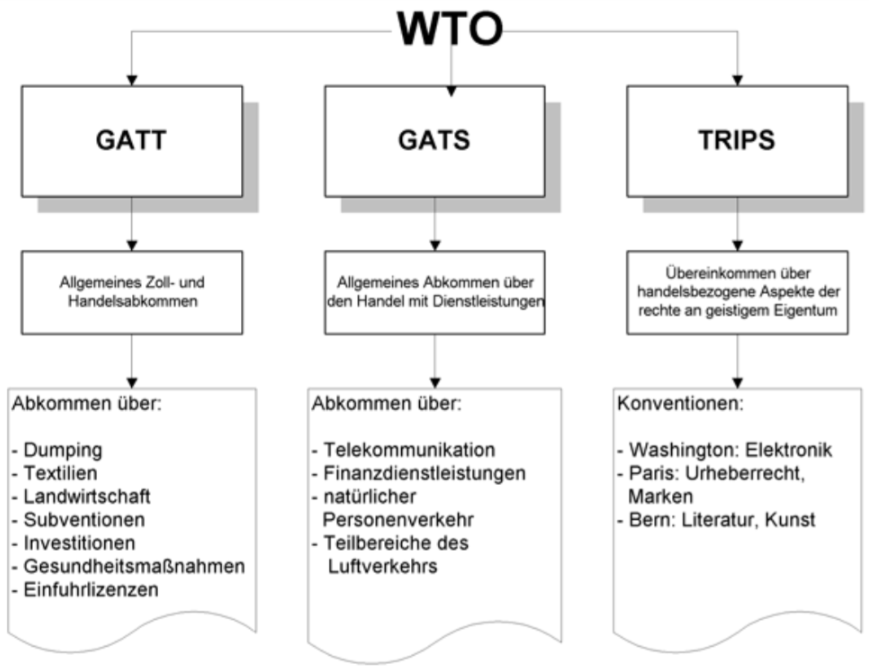
\includegraphics[width=\linewidth]{images/wto.png}
\end{minipage}%
\vspace{\baselineskip}
\textbf{OECD Organisation für Wirtschaftliche Zusammenarbeit und Entwicklung}
\begin{itemize}
	\item Ziele:
	\begin{itemize}
		\item beitragen zu einer optimalen Wirtschaftsentwicklung, hoher Beschäftigung und steigendem Lebensstandard
		\item Wirtschaftswachstum fördern
		\item Ausweitung des Welthandels auf multilateraler Basis
	\end{itemize}
	\item liberale, marktwirtschaftliche und effiziente Wirtschaftsordnung
	\item bei Arbeits- und Produktionsmärkten für den Abbau von Schranken und mehr Wettbewerb
	\item 35 Mitglieder
	\begin{itemize}
			\item fühlen sich der Demokratie und Marktwirtschaft verpflichtet 
			\item die meisten sind Länder mit hohem Pro-Kopf-Einkommen
	\end{itemize}
	\item 1961 als Nachfolgeorganisation der OEEC und des Marshallplans zum Wiederaufbau Europas gegründet
	\item OEEC: wirtschaftlicher Wiederaufbau, Zusammenarbeit in Europa
\end{itemize}
\vspace{\baselineskip}
\textbf{UNCTAD Konferenz der Vereinigten Nationen für Handel und Entwicklung}
\begin{itemize}
	\item ständiges Organ der Generalversammlung der UN
	\item Förderung des Handels zw. Ländern mit unterschiedlichem Entwicklungsstand
	\item bessere Verständigung Nord-Süd
	\item neue Weltwirtschaftsordnung erarbeiten
\end{itemize}
\vspace{\baselineskip}
\textbf{G7 Gruppe der Sieben}
\begin{itemize}
	\item informeller Zusammenschluss der zur Gründung bedeutendsten Industrienationen der westlichen Welt
	\item Forum zum Zweck, Fragen der Weltwirtschaft zu erörtern
	\item Deutschland, Frankreich, Italien, Japan, Kanada, Vereinigtes Königreich, USA (Europäische Kommission hat Beobachterstatus)
	\item 1975 etabliert, 1998 mit Russland zur G8, 2014 Russland wieder ausgeschlossen (Krim-Annexion)
\end{itemize}
\vspace{\baselineskip}
\textbf{G20 Gruppe der Zwanzig}
\begin{itemize}
	\item manchmal auch G21, G22 oder G20+
	\item Entwicklungs- und Schwellenländer
	\item 2003 gegründet
	\item führende Mitglieder: Brasilien, Indien, China, Türkei
	\item vor allem Themen aus der Landwirtschaft
	\item fordern Abbau von Agrarsubventionen und Aufhebung von Importbeschränkungen in Ländern wie der USA und in der EU
\end{itemize}
\clearpage
\pagebreak